%!TEX root = Funktionalanalysis - Vorlesung.tex


\section{Trennungssätze für konvexe Menge}


\begin{definition}
	Sei $X$ ein Vektorraum mit $A \subset X$. Die Abbildung 
		\[ p_{A} \colon X \rightarrow [0, \infty], ~ p_{A}(x) \coloneqq \inf \{ \lambda > 0 : \lambda x \in A \} \]
		hei{\ss}t Minkowski-Funktional von $A$ und $A$ hei{\ss}t \begriff{absorbierend}, falls $p_{A}(x) < \infty, \forall x \in X$, d.h. für alle $ x \in X$ gibt es ein $\lambda \geq 0$, sodass $x \in \lambda A$.
\end{definition}


\begin{beispiel}
	Für $A = U_{X}$ ist $p_{A}(x) = \| x \|$ $( \| x \| \leq \lambda \gdw x \in \lambda (U_{X})$.	
\end{beispiel}


\begin{prop} \label{prop:21.3}
	Sei $U \subset X$ konvex und $0$ innerer Punkt von $U$. Dann gilt
	\begin{enumerate}[label=\alph*\upshape)]
		\item Falls $\epsilon U_{X} \subset U \Rightarrow p_{U}(x) \leq \frac{1}{\epsilon} \| x \|$
		\item $p_{U}$ ist sublinear
		\item Ist $U$ offen, so ist $U = p_{U}^{-1}([0 , 1))$
	\end{enumerate}	
\end{prop}

\begin{beweis}
	\begin{enumerate}[label=\alph*\upshape)]
		\item $x \in \epsilon \cdot U_{X} \Rightarrow \frac{1}{\epsilon} \cdot x \in U_{X} \Rightarrow p_{U}(x) \leq \frac{1}{\epsilon} \cdot \| x \|$.
		\item $p_{U}(\lambda x ) = \lambda \cdot p_{U}(x)$ für $\lambda > 0$, denn 
			\[ (r \lambda) x \in U \gdw r(\lambda x) \in U \] 
			Zu $\epsilon > 0$ wähle $\lambda, \mu > 0$ mit  $\lambda \leq p_{U}(x) + \epsilon, ~\mu \leq p_{U}(y) + \epsilon$. Dann $\frac{x}{\lambda} \in U, \frac{y}{\mu} \in U$ 
			\[ \xRightarrow[]{Konv} \frac{\lambda}{\lambda + \mu} \left( \frac{x}{\lambda} \right) + \frac{\mu}{\mu + \lambda} \left( \frac{y}{\mu} \right) = \frac{x + y}{\lambda + \mu} \in U \]
			Somit ist $p_{U}(x + y) \leq \lambda + \mu \leq p_{U}(x) + p_{U}(y) + 2 \epsilon \text{ für alle } \epsilon > 0$.
		\item $x \in p_{U}^{-1}([0, 1]) \Rightarrow p_{U}(x) \leq 1$. Dann existiert ein $\lambda < 1$ mit $\frac{x}{\lambda} \in U$. Da $0 \in U$ und $U$ konvex ist, folgt
			\[ x = \lambda \left( \frac{x}{\lambda} \right) + (1 - \lambda) 0 \in U \]
			Sei umgekehrt $x \in U$. Da $U$ offen ist, gibt es $\epsilon > 0$ mit $x + \epsilon x \in U \Rightarrow p_{U}(x) \leq \frac{1}{1 + \epsilon}$.
	\end{enumerate}
\end{beweis}


\begin{satz}[1. Trennungssatz]
	Sei $X$ ein normierter Vektorraum, $V_{1}, V_{2} \subset X$ mit
	\begin{itemize}
		\item $V_{1}, V_{2}$ konvex, $V_{1} \cap V_{2} = \emptyset$
		\item $V_{1}$ offen,
	\end{itemize}
	dann gibt es ein $x' \in X'$ so, dass $\Re x'(v_{1}) < \Re x'(v_{2})$ für alle $v_{1} \in V_{1}, v_{2} \in V_{2}$.
\end{satz}

		\begin{figure}[H]
			\centering		
			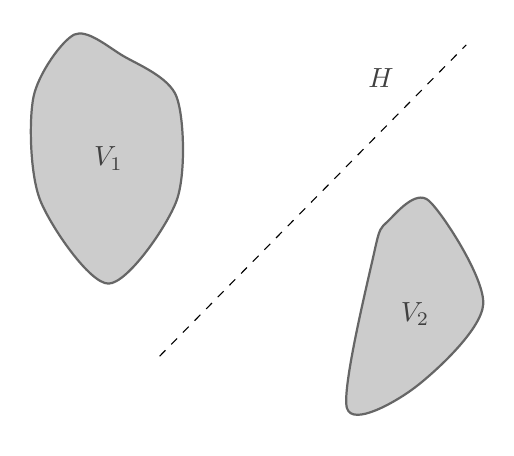
\begin{tikzpicture}
			 \begin{axis}[axis x line=none, axis y line=none]
				\addplot[mark=none, black!60, smooth cycle, thick, fill=gray!40] coordinates {(1,2) (2,1.6) (3,2) (3,2.5) (2.2, 2.7) (1.5, 2.8) (0.9, 2.5)};
				\node[black!75] at (axis cs:2,2.1) [anchor=south] {$V_1$};
				\addplot[dashed] coordinates {(2.75,1.25) (7.25,2.75)};
				\node[black!75] at (axis cs:6,2.5) [anchor=south] {$H$};
				
				\addplot[mark=none, black!60, smooth cycle, thick, fill=gray!40] coordinates {(5.5,1) (6.5,1.1) (7.5,1.5)  (6.7, 2) (6.1, 1.9) (5.9, 1.75)};
				\node[black!75] at (axis cs:6.5,1.35) [anchor=south] {$V_2$};
			 \end{axis}
			\end{tikzpicture}
		\end{figure}
	\[ H = \left\{ x : x'(x) = \inf_{v_{2} \in V_{2}} x'(v_{2}) \right\} \]

\begin{beweis}
	$(i)$ Sei $V_{2} = \{ 0 \}, \MdK = \MdR$. Wähle ein beliebiges $x_{0} \in V_{1}$ und setze $y_{0} = - x_{0}$. 
	\[ U \coloneqq \{ v - x_{0} : v \in V_{1} \} \text{ ist offen und konvex; außerdem: } 0 \in U, y_{0} \notin U \]
	Nach \hyperref[prop:21.3]{Prop. 21.3} gilt $p_{U}(y_{0}) \geq 1$ und $p_{U}(y) \leq C \| y \|$. Auf dem Untervektorraum $y = \ospan \{ y_{0} \}$ def $y' \colon Y \rightarrow \MdR, y'(t y_{0}) \coloneqq t p_{U}(y_{0})$ für $t \in \MdR$ ein Funktional. Dann gilt $y'(t y_{0}) \leq 0 \leq p_{U}(t y_{0})$ für $t < 0$, $y'(t y_{0}) = t p_{U}(y_{0}) = p_{U}(t y_{0})$ für $t \geq 0$ 
	\[ \Rightarrow y'(y) \leq p_{U}(y) \forall y \in Y \]
	Nach \hyperref[satz:20.3-HahnBanach]{Hahn-Banach} gibt es eine Fortsetzung $x' \colon X \rightarrow \MdR$ mit $x'(x) \leq p(x) \forall x \in X, x'$ ist linear und stetig, denn 
	\[ |x'(x)| = \max \{ | x'(x) | , | x'(-x) | \} \leq \max \{ p(x) , p(-x) \} \leq C \| x \| \]
	Für $x \in V_{1}$ gilt $x + y_{0} \in U$ und $x'(x) = x'(x + y_{0}) - x'(y_{0}) < 0$, denn mit \hyperref[prop:21.3]{Prop. 21.3} folgt
	\[ x'(y_{0}) = p(y_{0}) \geq 1 \quad \text{und} \quad  p(x + y_{0}) < 1, \text{ da } x + y_{0} \in U, x'(0) = 0 \]
	$(ii)$ Sei $V_{2} = \{ 0 \}, \MdK = \MdC$. Sei $X_{\MdR}$ der Vektorraum $X$ aufgefasst als reeller Vektorraum. Nach $(i)$ existiert ein $x'_{\MdR} \in X'_{\MdR}$ mit 
	\[ x'_{\MdR}(v_{1}) < \underbrace{x'_{\MdR}(v_{2}}_{= 0}  \]
	Wie im Beweis des \hyperref[satz:20.3-Hahn-Banach]{Satzes von Hahn-Banach}: $x'(x) \coloneqq x'_{\MdR}(x) - i x'_{\MdR}(-x) \Rightarrow x'$ $\MdC$-linear, stetig und $\Re x'(x) = x'_{\MdR}(x)$ \\
	$(iii)$ $V_{1}, V_{2}$ allgemein. Setze $W_{1} \coloneqq V_{1} - V_{2}$ konvex und offen $\left( W_{1} = \bigcup_{v_{1} \in V_{1}} \{ v_{1} - V_{2} \} \right)$.  \\
	Weiter ist $0 \in W_{1}$, denn $V_{1} \cap V_{2} = \emptyset$. \\
	Nach $(ii)$ gibt es ein $x' \in X'$ mit $\Re x'(v_{1} - v_{2}) < 0 \Rightarrow \Re x'(v_{1}) < \Re x'(v_{2})$ für $v_{1} \in V_{1}, v_{2} \in V_{2}$.
\end{beweis}

\begin{satz}[2. Trennungssatz]
	Sei $X$ ein normierter Raum, $V \subset X$ konvex und abgeschlossen. Für $x \notin V$ gibt es ein $x' \in X'$ mit:
		\[ \Re x'(x) < \inf \{ \Re x'(v) : v \in V \} \]	
\end{satz}


\newpage